\documentclass{article}
%%%%%%%%%%%%%%%%%%%%%%%%%%%%%%%%%%%%%%%%%%%%%%%%%%%%%%%
% GitHub Cheat Sheet
%%%%%%%%%%%%%%%%%%%%%%%%%%%%%%%%%%%%%%%%%%%%%%%%%%%%%%%

% Identificação
\newcommand{\pbtitulo}{\huge{\textbf{DataScience}}}
\newcommand{\pbversao}{1.0}

\usepackage{sty/cheatsheet}

\begin{document}

\begin{center}{\pbtitulo}\\
{\large Fernando Anselmo - Versão \pbversao}
\end{center}

\begin{multicols*}{3}

\tikzstyle{mybox} = [draw=contorno, fill=white, very thick,
    rectangle, rounded corners, inner sep=10pt, inner ysep=10pt]
\tikzstyle{fancytitle} =[fill=DarkBlue, text=white, font=\bfseries]

%------------ Data Science ---------------------
\begin{tikzpicture}
  \node [mybox] (box){%
    \begin{minipage}{0.3\textwidth} \vspace{0.5em}
 	  \begin{figure}[H]
	    \centering
	    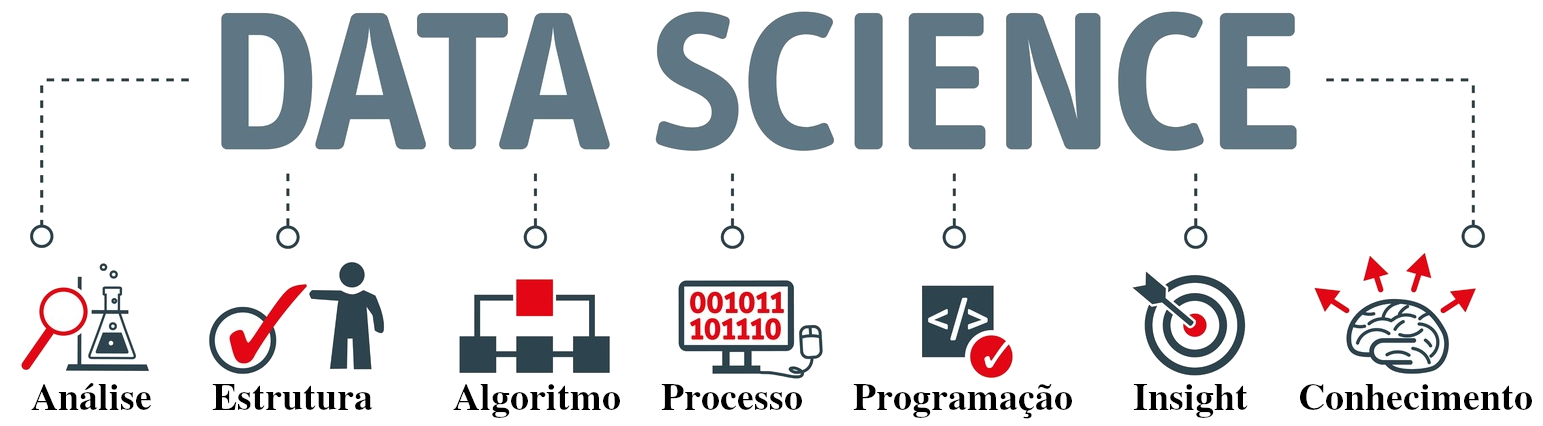
\includegraphics[width=1.0\textwidth]{imgDS/Data}
	  \end{figure}
	  \textbf{Cientistas de Dados} são responsáveis por: coletar os dados, limpar e organizar os dados, construir bases de treinamento e garantir que não ocorra \textit{overfitting}, construir algoritmos, gerar \textit{insights} e apresentá-los. \\[2mm]
	  \textbf{Habilidades em}: Estatística, entender do negócio e ter experiência no assunto, colaboração, resolução de problemas, ferramentas de visualização, bases de dados SQL e NoSQL, processamento de Big Data, Inteligência Artificial, Aprendizado de Máquina, Mineração de Dados, Linguagens de Programação, comunicação e criatividade. \\
	  \textbf{Habilidade Principal}: \textbf{Curiosidade}.
    \end{minipage}
  };  
  \node[fancytitle, right=10pt] at (box.north west) {Data Science};
\end{tikzpicture}

%------------ Análises ---------------
\begin{tikzpicture}
  \node [mybox] (box){%
    \begin{minipage}{0.3\textwidth} \vspace{0.5em}
	  \textbf{Descritiva} - responde: \aspas{o que aconteceu?} realizada com base em dados complementares e concorrentes. Necessita da Inteligência de Negócio. \\
  	  \textbf{Diagnóstica} - responde: \aspas{qual o motivo?} útil para determinar o sucesso/fracasso de qualquer ação com base nos dados. \\
  	  \textbf{Preditiva} - incita: \aspas{o que acontecerá?} extrapola a descritiva para prever uma tendência. \\
  	  \textbf{Prescritiva} - incita: \aspas{o que deve ser feito?} com base em uma estimativa informada do que acontecerá.
	\end{minipage}
  };
  \node[fancytitle, right=10pt] at (box.north west) {Análises};
\end{tikzpicture}

%------------ Linguagens ---------------
\begin{tikzpicture}
  \node [mybox] (box){%
    \begin{minipage}{0.3\textwidth} \vspace{0.5em}
	  Encarar a linguagem como uma ferramenta. \\
	  Pensar simples e consulte sempre. \\
	  Utilizar as bibliotecas, não reinventar a roda. \\
	  Documentar todo seu esforço. \\
	  Não focar em Orientação a Objetos, manter simples. \\
	  Não focar na tecnologia, muda constantemente.
    \end{minipage}
  };
  \node[fancytitle, right=10pt] at (box.north west) {Linguagens};
\end{tikzpicture}

%------------ Data Swamp/Lake ---------------
\begin{tikzpicture}
  \node [mybox] (box){%
    \begin{minipage}{0.3\textwidth} \vspace{0.5em}
      \textbf{Data Swamp} são todos os dados que entram, não possuem documentação nem padrão. \\
      \textbf{Data Lake} são os dados tratados (normalmente por um ETL como o Pentaho), estão em estado bruto e a disposição para serem explorados. Devem ser altamente acessíveis e passíveis de rápidas atualizações. 
      
    \end{minipage}
  };
  \node[fancytitle, right=10pt] at (box.north west) {Data Swamp/Lake};
\end{tikzpicture}

%------------ IA - ML ---------------------
\begin{tikzpicture}
  \node [mybox] (box){%
    \begin{minipage}{0.3\textwidth} \vspace{0.5em}
 	  \begin{figure}[H]
        \centering
        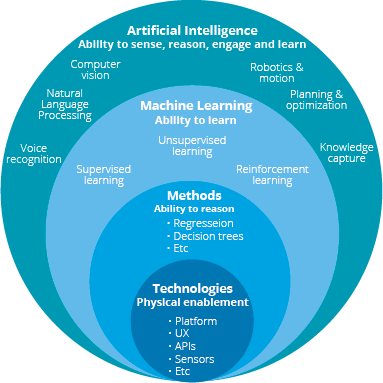
\includegraphics[width=1.0\textwidth]{imgDS/model}
      \end{figure}
    \end{minipage}
  };
  \node[fancytitle, right=10pt] at (box.north west) {IA \& ML};
\end{tikzpicture}

%------------ Big Data ---------------
\begin{tikzpicture}
  \node [mybox] (box){%
    \begin{minipage}{0.3\textwidth} \vspace{0.5em}
	  \textbf{Volume}: Quantidade. Escala acima de Petabytes. \\
	  \textbf{Velocidade}: Geração. Em tempo real, \textit{streaming} e \textit{batch}, entre servidores. \\
	  \textbf{Variedade}: Diferença. Estruturados, semi-estruturados, não estruturados e multi-fator. \\
	  \textbf{Veracidade}: São reais e podem ser comprovados. \\
	  \textbf{Valor}: Estatísticas, correlações, predições e hipóteses. \\
	  \textbf{Complexidade}: Alta dimensionalidade. \\
	  \textbf{Arquitetura}: Distribuída ou horizontal. \\
	  \textbf{Globalidade}: Variadas entradas de informação.
	\end{minipage}
  };
  \node[fancytitle, right=10pt] at (box.north west) {Big Data};
\end{tikzpicture}

%------------ Classificação e Regressão ---------------------
\begin{tikzpicture}
  \node [mybox] (box){%
	\begin{minipage}{0.3\textwidth} \vspace{0.5em}
  	  \textbf{Classificação}: prever um rótulo, a variável de resposta é do tipo categórica. Exemplos: Spam/Não, Doentes/Não, Cliente/Não. Algoritmos: KNN, Regressão Logística, SVM, Árvores de Decisão, XGBoost e Redes Neurais. \\
 	  \begin{figure}[H]
        \centering
        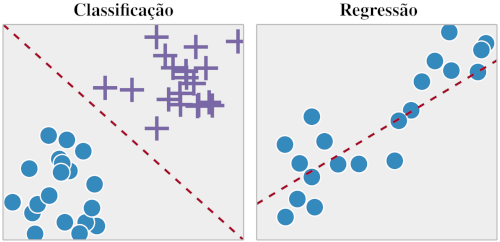
\includegraphics[width=1.0\textwidth]{imgDS/classReg}
      \end{figure}
  	  \textbf{Regressão}: prever uma quantidade, a variável de resposta é do tipo contínua. Exemplos: Estimativas de preço, tempo de uso de um serviço. Algoritmos: Regressão Linear, Regressão Polinomial.
	\end{minipage}
  };
  \node[fancytitle, right=10pt] at (box.north west) {Classificação e Regressão};
\end{tikzpicture}

%------------ Plataformas de Competição ---------------------
\begin{tikzpicture}
  \node [mybox] (box){%
	\begin{minipage}{0.3\textwidth} \vspace{0.5em}
	  \textbf{AICrowd} - \url{https://www.aicrowd.com} \\
	  \textbf{CodaLab} - \url{https://codalab.org} \\
	  \textbf{CrowdAnalytix} - \url{https://www.crowdanalytix.com} \\
	  \textbf{DataHack} - \url{https://www.analyticsvidhya.com} \\
	  \textbf{DrivenData} - \url{https://www.drivendata.org} \\
	  \textbf{HackerEarth} - \url{https://www.hackerearth.com} \\
	  \textbf{IDAO} - \url{https://idao.world} \\
	  \textbf{Iron Viz} - \url{https://www.tableau.com/iron-viz} \\
	  \textbf{Kaggle} - \url{https://www.kaggle.com/} \\
	  \textbf{MachineHack} - \url{https://analyticsindiamag.com} \\
	  \textbf{Tianchi} - \url{https://tianchi.aliyun.com} \\
	  \textbf{TopCoder} - \url{https://www.topcoder.com} \\
	  \textbf{Zindi} - \url{https://zindi.africa}
	\end{minipage}
  }; 
  \node[fancytitle, right=10pt] at (box.north west) {Plataformas de Competição};
\end{tikzpicture}

Outros Cartões: \url{https://github.com/fernandoans/publicacoes/tree/master/Sheet}

\end{multicols*}
\end{document}